\section{Parallelization evaluation}

Evaluating parallel algorithms requires an analysis of both time complexity, which quantifies the duration needed to complete a solution, and resource complexity, which measures the computational resources, such as processors and memory, required to achieve that time. 
These metrics provide essential insights into the scalability and efficiency of a parallel algorithm.

To analyze a parallel algorithm, we often represent its structure as a Directed Acyclic Graph. 
In this framework, nodes represent tasks, while edges indicate dependencies among tasks. 
Tasks that can be executed independently are concurrent, while parallel tasks are tasks that are executed simultaneously due to the availability of multiple processing resources.

\subsection{Algorithms evaluation}
Work ($W$) is a critical metric, representing the total number of operations performed by the algorithm. 
Unlike a sequential algorithm, a parallel algorithm's work may be higher due to communication overhead and other parallelization costs. 
The span ($S$), on the other hand, represents the longest dependency path, or the critical path, which defines the minimum time to complete the algorithm even if unlimited processors were available.
Together, these metrics allow us to derive parallelism ($P$), calculated as $P=\frac{W}{S}$, which measures the algorithm's efficiency in utilizing resources. 
\begin{table}[h!]
    \centering
    \begin{tabular}{|c|c|c|}
        \hline
        \textbf{Operation} & \textbf{Work (W)} & \textbf{Span (S)} \\
        \hline
        Single operation ($op$) & $W(op) = 1$ & $S(op) = 1$ \\
        \hline
        Sequential tasks ($e_1, e_2$) & $W(e_1, e_2) = W(e_1) + W(e_2)$ & $S(e_1, e_2) = S(e_1) + S(e_2)$ \\
        \hline
        Parallel tasks ($e_1 \parallel e_2$) & $W(e_1 \parallel e_2) = W(e_1) + W(e_2)$ & $S(e_1 \parallel e_2) = \max(S(e_1), S(e_2))$ \\
        \hline
    \end{tabular}
\end{table}
This average represents the number of processors that remain busy; however, the actual number of processors required for full-speed execution may need to be larger to avoid processor idleness.
\begin{figure}[H]
    \centering
    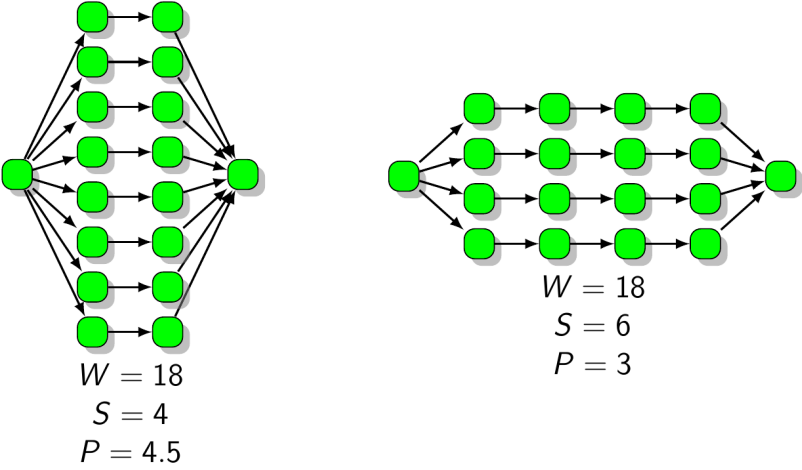
\includegraphics[width=0.75\linewidth]{images/pl.png}
    \caption{Examples of parallel algorithms}
\end{figure}
Effective parallel algorithm design balances the goal of minimizing work to reduce resource usage with the need to maximize parallelism by reducing the span. 
However, optimizing for parallelism may introduce additional communication and synchronization overhead, making it necessary to find a balance that minimizes both work and span as much as possible. 
This trade-off between work and parallelism requires careful consideration, as adding more parallelism can increase the complexity and overhead.

\subsection{Memory architectures}
The architecture of the memory system in parallel computers also impacts algorithm performance. 
In shared memory systems, processes can communicate through a common address space without explicit communication commands. 
This model simplifies parallel programming but poses challenges for maintaining data locality, which can slow performance when contention for shared resources increases. 
In distributed memory systems, each task has its own memory, requiring explicit communication between tasks. 
Though this approach is more complex, it improves data locality and is more scalable, particularly in large-scale systems.

A hybrid model combining MPI (Message Passing Interface) and OpenMP (Open Multi-Processing) offers flexibility by leveraging both distributed and shared memory advantages. 
For instance, MPI is often used for coarser-grained parallelism across CPUs, while OpenMP enables finer-grained parallelism within each multi-core CPU. 
In another approach, MPI can manage communication, while OpenMP focuses on parallelizing computation, allowing the system to handle different levels of parallelism efficiently.

Ultimately, evaluating parallel algorithms involves balancing algorithmic efficiency with architectural factors to achieve scalable performance across varying hardware configurations.
Effective parallelization depends on understanding these trade-offs and designing solutions that optimize both computational resources and processing time.